\documentclass[12pt, a4paper]{article}

\usepackage{graphicx, fullpage, hyperref, listings}
\usepackage{appendix, pdfpages, color}
\usepackage{tocloft}
\usepackage{amsmath}

\setlength\cftbeforesecskip{3pt}
\definecolor{MyLightYellow}{cmyk}{0,0.,0.2,0}
\interfootnotelinepenalty=500 

\setlength{\parindent}{0pt}
\setlength{\parskip}{7pt}
% \linespread{1.213}

\lstset{
  language=C++,
  columns=fullflexible,
  tabsize=4,
}

\title{
  
\includegraphics[width=0.6\textwidth]{LivUniCrest} \\
  Report on Assignment 1
}
\author{
  %\textcolor{red}{Student ID 201601082} \\ 
  \textcolor{red}{ELEC230}
}
\date{\today}


\begin{document}

\begin{titlepage}
  \maketitle
  \addtocontents{toc}{\protect\thispagestyle{empty}}

  \fbox{\begin{minipage}{0.9\linewidth} \footnotesize
     \begin{center} \textbf{Declaration} \end{center}
     I confirm that I have read and understood the University's definition of plagiarism and collusion from the Code of Practice on Assessment. I confirm that I have neither committed plagiarism in the completion of this work nor have I colluded with any other party in the preparation and production of this work. The work presented here is my own and in my own words except where I have clearly indicated and acknowledged that I have quoted or used figures from published or unpublished sources (including the web). I understand the consequences of engaging in plagiarism and collusion as described in the Code of Practice on Assessment (Appendix L).
  \end{minipage}}

\tableofcontents
\end{titlepage}

\section{Development Environment}
\begin{itemize}
  \item Language standard: C++17
  \item Compiler: Clang9
  \item Debugger: LLDB9
  \item Dependencies:
    \subitem libc++
\end{itemize}

\section{Part A}
\subsection{Feature List}
\begin{itemize}
  \item a user defined class which models a two dimensional polygon
  \item translate the polygon by a translation vector
  \item rotate the polygon around certain point by certain radian
\end{itemize}

\subsection{Feature Design}
Class structure of 2D regular polygon whose centorid is on the origin is specified in the assignment description.

\textbf{point:} Model a 2D point by a struct which has two fields: x and y

\textbf{vector:} Model a 2D vector by a struct which has two fields: x and y

\textbf{constructor:} To ensure the base of regular polygon lies horizontally, first define a point (0, -radius), then rotate it by $\frac{2\pi}{\text{number of vertices}} \times \frac{1}{2}$. This yields a point which is a vertex on the horizontal base line of the polygon. A vertex of a regular polygon can be calculated by rotating its neighbouring vertices around the origin by $\frac{2\pi}{\text{number of vertices}}$. Here a rotation matrix is used to calculate the point after rotating around the origin:
\begin{equation} 
  \begin{bmatrix}
    \text{unkown vertex}_x \\
    \text{unkown vertex}_y \\
  \end{bmatrix}
  =
  \begin{bmatrix}
    \cos\theta & -\sin\theta \\
    \sin\theta & \cos\theta \\
  \end{bmatrix}
  \begin{bmatrix}
    \text{neighbouring vertex}_x \\
    \text{neighbouring vertex}_y \\
  \end{bmatrix}
\end{equation}

Defualt constructor is deleted for safety purpose.

\textbf{translate:} Pass the pre-defined vector struct as a translation vector into the method. Inside the method, simply add the tanslation vector on the origin vertices using iterator.

\textbf{rotate:} Pass the pre-defined point struct as a centre of rotation into the method. Pass a double type rotation radian. Transfer points so that their centre of rotation matches the origin, then rotate each point by a rotation matrix, finally transfer points back to their original place:
\begin{equation} 
  \begin{bmatrix}
    x \\
    y \\
  \end{bmatrix}
  =
  \begin{bmatrix}
    \cos\theta & -\sin\theta \\
    \sin\theta & \cos\theta \\
  \end{bmatrix}
  \begin{bmatrix}
    vertex_x - \textit{centre of rotation}_x \\
    vertex_y - \textit{centre of rotation}_y \\
  \end{bmatrix}
  +
  \begin{bmatrix}
    \textit{centre of rotation}_x \\
    \textit{centre of rotation}_y \\
  \end{bmatrix}
\end{equation}

\subsection{Feature Implementation}
Refer to the source code.

\subsection{Test}
To reduce the workload, neither a unit testing framework nor comprehensive test criteria is used. Only a simple demo is provided in the main. Please refer to the source code.

\begin{figure}[htbp]
  \begin{centering}
    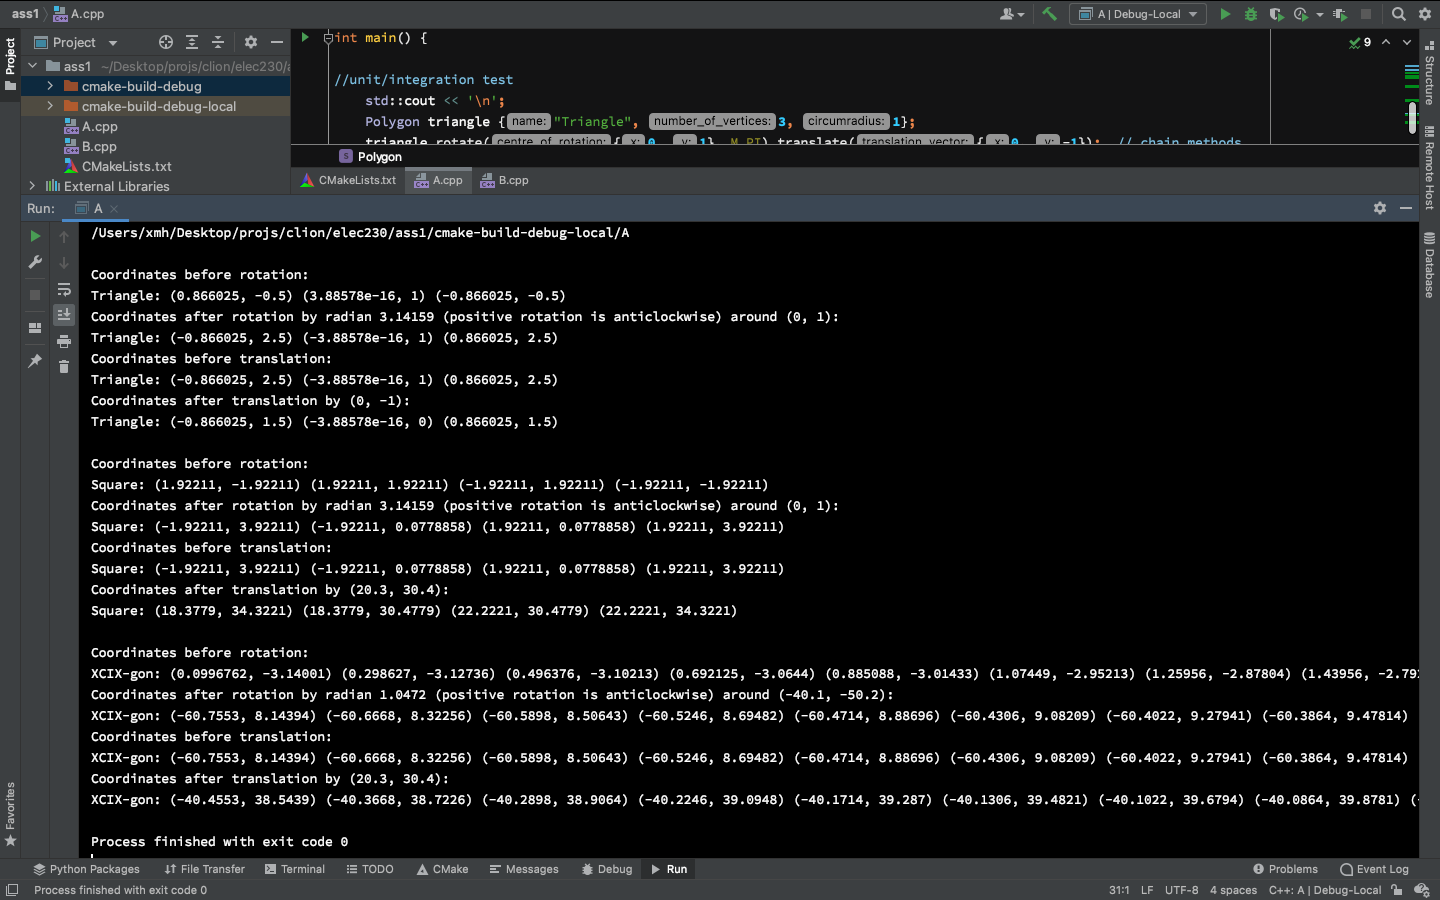
\includegraphics[width=1\textwidth]{A_results}
    \caption{Part A results (demo)}
  \end{centering}
  \label{fig:A_demo}
\end{figure}

\section{Part B}
\subsection{Feature List}
\begin{itemize}
  \item a abstract base class (ABC) which models a three dimensional polygon with tanslate and rotate as two pure virtual functions
  \item in three dimension, rotate or translate the polygon in xy or xz or yz plane only
  \item batch-rotate and batch-translate several polygon instances which based on the same ABC via pointer
\end{itemize}

\subsection{Feature Design}
\begin{figure}[htbp]
  \begin{centering}
    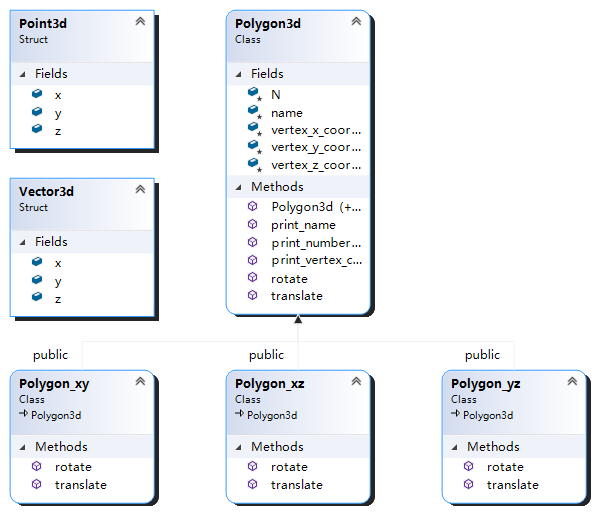
\includegraphics[width=0.7\textwidth]{B_UML}
    \caption{Part B UML class diagram}
  \end{centering}
  \label{fig:B_UML}
\end{figure}

\textbf{point:} Model a 3D point by a struct which has three fields: x, y, and z

\textbf{vector:} Model a 3D vector by a struct which has three fields: x, y, and z

\textbf{constructor:} Pass a series of vertices via \lstinline{std::initializer_list<Point3d>}, and map it to the assignment-defiend class fields by std::transform. Other fields' value can be simply passed in by value then initialised in the constructor initialise list. Delete the defualt constructor for safety purpose.
\begin{lstlisting}[frame=single, breaklines]
Polygon3d() = delete;
Polygon3d(std::string name, std::initializer_list<Point3d> const& vertices)
    : name {std::move(name)}
{
    std::transform(vertices.begin(), vertices.end(), std::back_inserter(vertex_x_coordinates), [](Point3d const& point3D){return point3D.x;});
    // similar as the above statement
}
\end{lstlisting}

\textbf{translate:} Although a three dimension vector is passed into the method, one dimension is ignored without any warning message to peform the translation.

\textbf{rotate:} One dimension of three dimension is ignored without any warning message to peform the rotation.

\textbf{batch-translate/rotate:} Use \lstinline{std::initializer_list<ABC*>} to form an array of raw pointers whose type are the ABC. Then iterate through the array to do batches.
\begin{lstlisting}[frame=single, breaklines]
for (auto polygon3d : std::initializer_list<Polygon3d*>{&xy, &xz, &yz}) {
    polygon3d->translate(translation_vector);
    polygon3d->rotate(centre_of_rotation, radian);
}
\end{lstlisting}

\subsection{Feature Implementation}
Refer to the source code.

\subsection{Test}
To reduce the workload, neither a unit testing framework nor comprehensive test criteria is used. Only a simple demo is provided in the main. Please refer to the source code.

\begin{figure}[htbp]
  \begin{centering}
    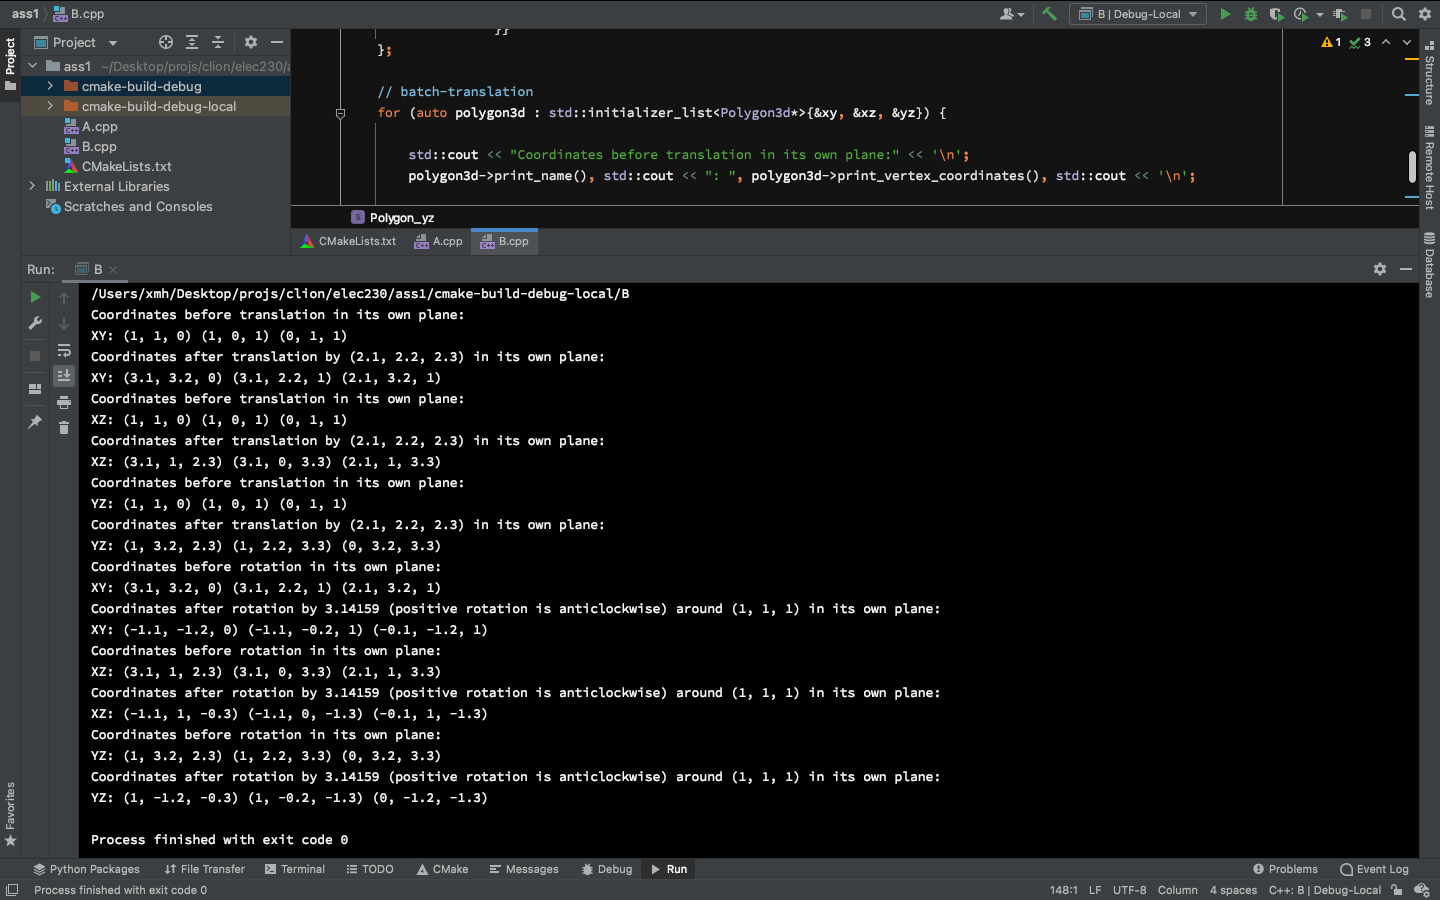
\includegraphics[width=1\textwidth]{B_results}
    \caption{Part B results (demo)}
  \end{centering}
  \label{fig:B_demo}
\end{figure}

\end{document}
